\fancyhead[L]{\textbf{\textsf{44}}}
\fancyhead[R]{\textbf{\textsf{\color{stewartcyan}CHƯƠNG 1}}\quad \textsf{Hàm số và Mô hình}}

\noindent
\begin{minipage}[t]{0.485\textwidth}
\textbf{\textsf{\color{stewartcyan}33--34}}\quad Tìm (a) $f + g$, (b) $f - g$, (c) $fg$, và (d) $f/g$ cùng tập xác định của chúng.

\medskip
\noindent
\textbf{33.} $f(x) = \sqrt{25 - x^2}, \quad g(x) = \sqrt{x + 1}$

\medskip
\noindent
\textbf{34.} $f(x) = \dfrac{1}{x - 1}, \quad g(x) = \dfrac{1}{x} - 2$

\vspace{0.8ex}
\noindent{\color{stewartcyan}\rule{\linewidth}{0.6pt}}
\vspace{0.8ex}

\noindent
\textbf{\textsf{\color{stewartcyan}35--40}}\quad Tìm các hàm số (a) $f \circ g$, (b) $g \circ f$, (c) $f \circ f$, và (d) $g \circ g$ cùng tập xác định của chúng.

\medskip
\noindent
\textbf{35.} $f(x) = x^3 + 5, \quad g(x) = \sqrt[3]{x}$

\medskip
\noindent
\textbf{36.} $f(x) = \dfrac{1}{x}, \quad g(x) = 2x + 1$

\medskip
\noindent
\textbf{37.} $f(x) = \dfrac{1}{\sqrt{x}}, \quad g(x) = x + 1$

\medskip
\noindent
\textbf{38.} $f(x) = \dfrac{x}{x + 1}, \quad g(x) = 2x - 1$

\medskip
\noindent
\textbf{39.} $f(x) = \dfrac{2}{x}, \quad g(x) = \sin x$

\medskip
\noindent
\textbf{40.} $f(x) = \sqrt{5 - x}, \quad g(x) = \sqrt{x - 1}$

\vspace{0.8ex}
\noindent{\color{stewartcyan}\rule{\linewidth}{0.6pt}}
\vspace{0.8ex}

\noindent
\textbf{\textsf{\color{stewartcyan}41--44}}\quad Tìm $f \circ g \circ h$.

\medskip
\noindent
\textbf{41.} $f(x) = 3x - 2, \quad g(x) = \sin x, \quad h(x) = x^2$

\medskip
\noindent
\textbf{42.} $f(x) = |x - 4|, \quad g(x) = 2^x, \quad h(x) = \sqrt{x}$

\medskip
\noindent
\textbf{43.} $f(x) = \sqrt{x - 3}, \quad g(x) = x^2, \quad h(x) = x^3 + 2$

\medskip
\noindent
\textbf{44.} $f(x) = \tan x, \quad g(x) = \dfrac{x}{x - 1}, \quad h(x) = \sqrt[3]{x}$

\vspace{0.8ex}
\noindent{\color{stewartcyan}\rule{\linewidth}{0.6pt}}
\vspace{0.8ex}

\noindent
\textbf{\textsf{\color{stewartcyan}45--50}}\quad Biểu diễn hàm số đã cho dưới dạng $f \circ g$.

\medskip
\noindent
\begin{minipage}[t]{0.48\linewidth}
\textbf{45.} $F(x) = (2x + x^2)^4$
\end{minipage}\hfill
\begin{minipage}[t]{0.48\linewidth}
\textbf{46.} $F(x) = \cos^2 x$
\end{minipage}

\medskip
\noindent
\begin{minipage}[t]{0.48\linewidth}
\textbf{47.} $F(x) = \dfrac{\sqrt[3]{x}}{1 + \sqrt[3]{x}}$
\end{minipage}\hfill
\begin{minipage}[t]{0.48\linewidth}
\textbf{48.} $G(x) = \sqrt[3]{\dfrac{x}{1 + x}}$
\end{minipage}

\medskip
\noindent
\begin{minipage}[t]{0.48\linewidth}
\textbf{49.} $v(t) = \sec(t^2)\tan(t^2)$
\end{minipage}\hfill
\begin{minipage}[t]{0.48\linewidth}
\textbf{50.} $H(x) = \sqrt{1 + \sqrt{x}}$
\end{minipage}

\vspace{0.8ex}
\noindent{\color{stewartcyan}\rule{\linewidth}{0.6pt}}
\vspace{0.8ex}

\noindent
\textbf{\textsf{\color{stewartcyan}51--54}}\quad Biểu diễn hàm số đã cho dưới dạng $f \circ g \circ h$.

\medskip
\noindent
\begin{minipage}[t]{0.48\linewidth}
\textbf{51.} $R(x) = \sqrt{\sqrt{x} - 1}$
\end{minipage}\hfill
\begin{minipage}[t]{0.48\linewidth}
\textbf{52.} $H(x) = \sqrt[8]{2 + |x|}$
\end{minipage}

\medskip
\noindent
\begin{minipage}[t]{0.48\linewidth}
\textbf{53.} $S(t) = \sin^2(\cos t)$
\end{minipage}\hfill
\begin{minipage}[t]{0.48\linewidth}
\textbf{54.} $H(t) = \cos(\sqrt{\tan t + 1})$
\end{minipage}

\vspace{0.8ex}
\noindent{\color{stewartcyan}\rule{\linewidth}{0.6pt}}
\vspace{0.8ex}

\noindent
\textbf{\textsf{\color{stewartcyan}55--56}}\quad Sử dụng bảng giá trị để tính từng biểu thức.

\medskip
\begin{center}
\renewcommand{\arraystretch}{1.25}
\begin{tabular}{|c|c|c|c|c|c|c|}
\hline
\rowcolor{gray!10}
$x$ & 1 & 2 & 3 & 4 & 5 & 6 \\
\hline
$f(x)$ & 3 & 1 & 5 & 6 & 2 & 4 \\
\hline
$g(x)$ & 5 & 3 & 4 & 1 & 3 & 2 \\
\hline
\end{tabular}
\end{center}

\medskip
\noindent
\textbf{55.}
\begin{tabular}[t]{ll}
(a) $f(g(3))$ & (b) $g(f(2))$ \\
(c) $(f \circ g)(5)$ \hspace{2em} & (d) $(g \circ f)(5)$
\end{tabular}
\end{minipage}%
\hfill
\begin{minipage}[t]{0.485\textwidth}
\noindent
\textbf{56.}
\begin{tabular}[t]{ll}
(a) $g(g(g(2)))$ & (b) $(f \circ f \circ f)(1)$ \\
(c) $(f \circ f \circ g)(1)$ \hspace{2em} & (d) $(g \circ f \circ g)(3)$
\end{tabular}

\vspace{0.8ex}
\noindent{\color{stewartcyan}\rule{\linewidth}{0.6pt}}
\vspace{0.8ex}

\noindent
\textbf{57.} Sử dụng đồ thị đã cho của $f$ và $g$ để tính từng biểu thức, hoặc giải thích vì sao biểu thức không xác định.

\medskip
\noindent
\begin{tabular}{lll}
(a) $f(g(2))$ & (b) $g(f(0))$ & (c) $(f \circ g)(0)$ \\
(d) $(g \circ f)(6)$ \hspace{1.5em} & (e) $(g \circ g)(-2)$ \hspace{1.5em} & (f) $(f \circ f)(4)$
\end{tabular}

\begin{center}
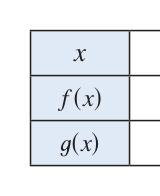
\includegraphics[width=0.65\linewidth]{images/p0079_fig1.png}
\end{center}

\noindent
\textbf{58.} Sử dụng đồ thị đã cho của $f$ và $g$ để ước lượng giá trị của $f(g(x))$ với $x = -5, -4, -3, \dots, 5$. Dùng các giá trị ước lượng này để phác thảo đồ thị của $f \circ g$.

\begin{center}
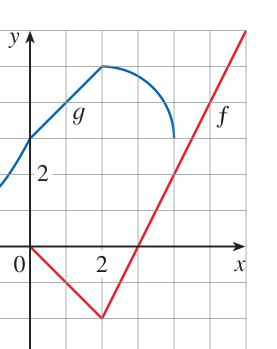
\includegraphics[width=0.65\linewidth]{images/p0079_fig2.png}
\end{center}

\noindent
\textbf{59.} Một viên đá được thả xuống hồ, tạo ra một gợn sóng hình tròn lan rộng ra phía ngoài với tốc độ $60\text{ cm/s}$.
\begin{enumerate}[label=(\alph*),leftmargin=1.8em,itemsep=0.2ex]
    \item Biểu diễn bán kính $r$ của đường tròn này theo hàm số của thời gian $t$ (tính bằng giây).
    \item Nếu $A$ là diện tích của hình tròn này dưới dạng hàm số của bán kính, hãy tìm $A \circ r$ và giải thích ý nghĩa thực tế của nó.
\end{enumerate}

\medskip
\noindent
\textbf{60.} Một quả bóng hình cầu đang được bơm căng và bán kính của nó tăng lên với tốc độ $2\text{ cm/s}$.
\begin{enumerate}[label=(\alph*),leftmargin=1.8em,itemsep=0.2ex]
    \item Biểu diễn bán kính $r$ của quả bóng theo hàm số của thời gian $t$ (tính bằng giây).
    \item Nếu $V$ là thể tích của quả bóng dưới dạng hàm số của bán kính, hãy tìm $V \circ r$ và giải thích ý nghĩa thực tế của nó.
\end{enumerate}

\medskip
\noindent
\textbf{61.} Một con tàu đang di chuyển với vận tốc $30\text{ km/h}$ song song với một bờ biển thẳng. Con tàu cách bờ biển $6\text{ km}$ và đi ngang qua một ngọn hải đăng vào đúng buổi trưa.
\begin{enumerate}[label=(\alph*),leftmargin=1.8em,itemsep=0.2ex]
    \item Biểu diễn khoảng cách $s$ giữa ngọn hải đăng và con tàu theo hàm số của quãng đường $d$ mà tàu đã đi được kể từ buổi trưa; nghĩa là tìm hàm số $f$ sao cho $s = f(d)$.
    \item Biểu diễn $d$ theo hàm số của thời gian $t$ đã trôi qua kể từ buổi trưa; nghĩa là tìm hàm số $g$ sao cho $d = g(t)$.
    \item Tìm $f \circ g$. Hàm số hợp này biểu thị điều gì?
\end{enumerate}
\end{minipage}